

\chapter{Mapping on superconducting quantum processors}
\label{sec:org0c87802}

In this chapter we describe the setup in which we focused on.
Although the work done is general and it could serve to any quantum technology we limit our studies on the SC-17 chip constrains.
We will explain the mapping model and the metrics used in the work.

\section{Constraints of the Surface-17 chip}
\label{sec:org168a66d}
\subfile{chapters/constraints}

\section{Mapping model}
\label{sec:org19dc500}
In order to map quantum circuits on the superconducting quantum chip we will use the mapping model developed in our group.
A mapping algorithm or mapper is an algorithm able to find a mapping solution given a quantum circuit and the target device constraints.
We consider that a mapper is subdivided in three tasks: scheduler, initial placement and routing, as described in the \url{chapter-2.org} section.
Our procedure is modular, although the flow is restricted to the one described below.
The mapper is fully adaptable to any device constrain.
It also offers two different kinds of schedulers and three router possibilities, as well as the option of running or not the initial placement and another options related to the chip constrains.
We believe this solution will aid researchers to investigate the best mapping, with different configurations.
The mapping model works as follows.

\subsection{Initial placement}
\label{sec:org4fe48f6}

Once the mapper knows the qubits required, the mapper will try to find the best initial placement for the given circuit.
First, it will check the first set of two-qubit gates and their target qubits.
If those qubits are not NN, it will initiate an Integer Liner Programming (ILP) algorithm \cite{Lao_2018} to find the optimal initial placement.
The one which requires the minimum number of qubit movements.


\subsection{Router}
\label{sec:org18105df}

Our router inspects all the gates, one by one, looking for non-NN qubits interactions.
Whenever the router finds one, it will insert the SWAP operations (decomposed or not decomposed) required to follow the selected path by the router.
A different path is generated depending on the router option that was selected by the user.
Although, all of them will try to extend minimally the depth of the circuit.
They always choose the path base on the latency or, what is the same, how well the SWAPs interleave with previous operations.
There are three router options:

\begin{enumerate}
\item \texttt{base} finds all the shortest paths and selects one of them randomly. The shortest paths are calculated based on the Manhattan distance, counting the number of steps that the qubits will need to move.
\item \texttt{minextend} finds all the shortest paths as well, but selects the one that would combine the SWAPs extending minimally the gate duration.
\item The \texttt{minextendrc} approach is exactly the same as the second one, but taking into account the chip constraints while mapping. It will select one of the best paths that would interleave the least with the constraints.
\end{enumerate}


\subsection{Scheduler}
\label{sec:org2ec75f3}

The RC-scheduler will finally scheduled the circuit using either an ALAP or an ASAP approach, depending on the user requirements.
It will take into account the chip parallelism constraints, as the ones described in \ref{sec:org168a66d}, scheduling in parallel only the possible operations
.

One downside factor regarding this methodology is that the mapper only takes into account one gate every time.
It does not look ahead in order to decide the best path for next iterations.
Or, what is the same, it does not always find the best mapping solution.
This limitation comes from the fact that, the more steps you are looking ahead while mapping, the more computationally complex will the mapper be.
We highlight that the mapping problem is an NP problem \cite{Siraichi_2018}.
Therefore, this method represents a viable solution, although a lot of future work should be done.

\section{New Mapping Metrics}
\label{sec:org27990de}
As mentioned in the \url{chapter-2.org} section in the second chapter, we name \emph{mapping metrics} to those metrics used to assert the quality of a mapper and that are also used by the mapper algorithm as an heuristic.
In this section we will review the common metrics as the \textbf{number of SWAPs} or the \textbf{latency}, but we will also define -- and study in more detail -- some new mapping metrics that we incorporated, \textbf{probability of success} and \textbf{Quantum Volume}.

\subsection{Probability of success and fidelity}
\label{sec:org0c7b2c2}

\begin{figure}
    \centering

\resizebox{0.3\textwidth}{!}{
   \Qcircuit @C=1em @R=.7em {
&&&&&\mbox{fidelity}&&&&\mbox{prob. success}\\
&&&&&&&&&\\
\lstick{a} & \targ & \qw & \qw & \qw & \qw \ar@{.}[]+<0.75em,1em>;[d]+<0.75em,-9em> & \meter \ar@{.}[]+<2em,1em>;[d]+<2em,-9em> & \rstick{0} \qw&&\\
\lstick{b} & \ctrl{-1} & \targ & \qw & \qw & \qw & \meter & \rstick{0} \qw&&\\
\lstick{c} & \qw & \ctrl{-1} & \targ & \qw & \qw & \meter & \rstick{0} \qw&&\\
\lstick{d} & \qw & \qw & \ctrl{-1} & \targ & \qw & \meter & \rstick{0} \qw&&\\
\lstick{e} & \qw & \qw & \qw & \ctrl{-1} & \targ & \meter & \rstick{0} \qw&&\\
\lstick{f} & \qw & \qw & \qw & \qw & \ctrl{-1} & \meter & \rstick{1} \qw&&
}
}
\caption{Example of the fidelity and probability of success calculation in the Gray encoder quantum circuit}
\label{fig:latency_swaps_ex_orig}
\end{figure}

We define probability of success as the probability of having the correct or expected results after running and measuring several times a quantum algorithm.
For instance, if the expected result of an algorithm is \texttt{0100} and the results are either \texttt{0001} or \texttt{1111} we will get a failure.
We will only get a success if the algorithm returns \texttt{0100}.
Then, in the previous example, if we get \texttt{0001}, \texttt{0100} and \texttt{1111} as results after running the algorithm three times the resulting probability of success will be \(\frac{1}{3}\).
This model was chosen because it is one of the most practical ways to include the measurement gate into the error analysis.
But, at the same time, we aware that this metric have a limitation: it cannot assert -- in just one run -- the success of an algorithm that ideally returns a quantum state different that either the ground or the excited state.
Once a quantum state is measured it collides in either ground or excited.
In order to extract the complete quantum state, several runs of the circuit should be done, inheriting the results as a probabilistic distribution or histogram.
For a state as \(0.3 | 0 \rangle + 0.7 | 1 \rangle\), after several measurements, we will get \texttt{0} a 30\% of the times and \texttt{1} 70\% of the times.
Accordingly, in order to calculate the probability of success, we will need to compare histograms instead of only one measured result.

Although not taking into account the measurement, the quantum fidelity metric is related with the probability of success.
Both compare two quantum states, but, while the success of an algorithm is a boolean metric -- either success or failure --, the fidelity returns a number of how different the states are.
How far is one state from the other.
As an analogy, if we consider the quantum states as vectors, the fidelity would be the dot product between them.
However, the fidelity between orthogonal states -- states that differ in rotations around the x-axis as \(| 0100 \rangle\), \(| 0001 \rangle\) and \(| 1111 \rangle\) -- is also 0.
In eq. \ref{eq:orge3c164e} the fidelity formula is shown to understand its behaviour.

\begin{equation}
\label{eq:orge3c164e}
{\displaystyle F(\rho ,\sigma )=\left(\operatorname {Tr} {\sqrt {{\sqrt {\rho }}\sigma {\sqrt {\rho }}}}\right)^{2},}
\end{equation}

where \(\rho =\sum _{i}p_{i}|i\rangle \langle i|\) and \(\sigma =\sum _{i}q_{i}|i\rangle \langle i|\).
These states are named \textbf{mixed states} and they are defined as the weighted sum of different pure states.
This is the general case in order to calculate the fidelity in any case.
But, for a situation with one of the states as pure state (\({\displaystyle \rho =|\psi _{\rho }\rangle \!\langle \psi _{\rho }|}\)) the calculation of fidelity reduces its complexity as it can be understood from eq. \ref{eq:org2703857}.
Eq. \ref{eq:org1f331e2} the next step of simplicity, the one in which both states are pure (\({\displaystyle \rho =|\psi _{\rho }\rangle \!\langle \psi _{\rho }|}, {\displaystyle \sigma =|\psi _{\sigma }\rangle \!\langle \psi _{\sigma }|} {\displaystyle \sigma =|\psi _{\sigma }\rangle \!\langle \psi _{\sigma }|}\)).


\begin{equation}
\label{eq:org2703857}
{\displaystyle F(\rho ,\sigma )=\operatorname {Tr} \left[{\sqrt {|\psi _{\rho }\rangle \langle \psi _{\rho }|\sigma |\psi _{\rho }\rangle \langle \psi _{\rho }|}}\right]^{2}=\langle \psi _{\rho }|\sigma |\psi _{\rho }\rangle \operatorname {Tr} \left[{\sqrt {|\psi _{\rho }\rangle \langle \psi _{\rho }|}}\right]^{2}=\langle \psi _{\rho }|\sigma |\psi _{\rho }\rangle .}
\end{equation}

\begin{equation}
\label{eq:org1f331e2}
{\displaystyle F(\rho ,\sigma )=|\langle \psi _{\rho }|\psi _{\sigma }\rangle |^{2}}
\end{equation}




In our study, we will use both metrics in order to calculate the amount of errors that arise from an algorithm.
As soon as fidelity is not taking into account the measurement errors, it is common that both metrics differ completely.
It could be the case that a quantum state is erroneous before the measurement and, then, due to the error added from the measurement the erroneous state would flip and converge into the expected state.
At the same time, a correct quantum state could be measured wrongly due to the measurement errors.

\subsection{Quantum Volume}
\label{sec:org3029336}

Given the different hardware implementations and technologies in Quantum Computation (superconducting, ion-trap, spin qubits, \ldots{}), it is often difficult to benchmark the usefulness or power of quantum systems. 
A \textbf{hardware-independent measure} is required to depict whether a device is able to run a quantum circuit or not.
Here is where the Quantum Volume metric appears on the scene.

The aim of Quantum Volume is to quantify the computational power of quantum devices. 
Consequently we will use it as a metric to measure the runnability of the quantum algorithms and the quantum devices -- \emph{\textbf{"can this algorithm be run in a given device?"}}.
While the device is the basis of the Quantum Volume metric, we fix our attention on the circuit.
Our purpose is to assert how the mapping procedure affects the runnability of a given circuit and to study how the Quantum Volume is related to the probability of success.

\begin{enumerate}
\item Definition
\label{sec:org6ff511c}

In this section, we define the Quantum Volume metric as well as the insights and ideas motivated by its capabilities

\begin{enumerate}
\item Hardware parameters
\label{sec:org0eaa33d}

The Quantum Volume metric considers that a quantum computer's performance mainly depends on the next hardware specifications:

\begin{itemize}
\item \(N\). The number of physical qubits
\item Quantum chip topology. The connectivity between qubits
\item Maximum number of sequential gates with correctable errors. The number of gates that can be applied before errors or decoherence mask the result
\item Gate set. Available hardware gate set
\item Maximum number of parallel operations. Number of operations that can be run in parallel
\end{itemize}

\item Definitions and metrics
\label{sec:org13428d2}

In order to understand the metric of Quantum Volume, some concepts need to be defined first. 
In this section we offer the inferred definitions from \cite{Bishop_2017,Moll_2018} that are part of the rationale of Quantum Volume.


\begin{description}
\item[{Model algorithm.}] In the literature, Bishop et al. use the term \emph{model algorithm} in \cite{Bishop_2017} to refer to a depth-one circuit, "constructed by random 2-qubit unitary matrix chosen uniformly over \(SU (4)\) on a random pairing of the qubits". Or, what is the same, the \emph{model algorithm} is a \emph{circuit unit} of depth one defined by a combination of any single- or two-qubit gates. The mapping requirements of the device and the mapping quality is included as well. In the case that a two-qubit gate force any qubit to be routed, the gate additions will be included in the \emph{model algorithm}. Therefore, we can say that it is device specific, as soon as it takes into account the constraints from it.
\end{description}

\begin{figure}[htbp]
\centering
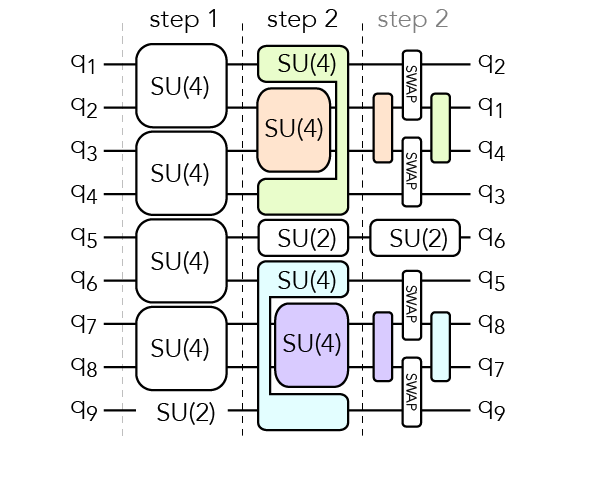
\includegraphics[width=0.7\textwidth]{figures/model_algorithm.png}
\caption{\label{fig:org31004c0}
Model algorithm example from \cite{Moll_2018}. Each step represents a possible combination of gates considered as \emph{model algorithm}. Notice that step 2 requires a mapping process that is shown afterwards.}
\end{figure}


\begin{description}
\item[{Active qubits (\(\textbf{n}\))}] Number of active qubits in a device of \(N\) qubits for a given algorithm.
\end{description}


\begin{description}
\item[{Effective error rate (\(\epsilon_{eff} \sim 1/(d(N) n)\)).}] It defines how well a device can implement arbitrary pairwise interactions between qubits. \(\epsilon_{eff}\) is the error rate per \emph{model algorithm}, an averaged error over many realizations of depth-one circuits conformed with random combinations of single- and two-qubit gates. It encapsulates errors of both single- and two-qubit gates. And it depends not only on the gate error rates, but also on the sophistication of the scheduling algorithm responsible of mapping the \emph{model algorithm} to the hardware.

\item[{Achievable circuit depth (\(d(N) \simeq \frac{1}{N \epsilon_{eff}}\))}] Maximum circuit depth for which the results, after running it on some device, are correctable and useful.
\end{description}

\begin{description}
\item[{(General) Quantum Volume (\(\tilde{V}_Q = min (N, d(N))^2\))}] quantifies the space-time volume occupied by a \emph{model algorithm} with random two-qubit gates that can be reliably executed on a given device.
\end{description}

\item Runnability
\label{sec:org03b929e}

After understading the concept of Quantum Volume, we derived some insights and we had ideas motivated by the possibilities that this new metric offers. 
We define the \textbf{runnability} of a given quantum circuit on a device based on the separation of the concepts of \emph{device} Quantum Volume (\(V_Q\)) and \emph{algorithm} Quantum Volume (\(V^a_Q\)).


\begin{enumerate}
\item Quantum Volume of a device
\label{sec:org52b9efe}

Following \cite{Bishop_2017,Moll_2018}, we can expand the Quantum Volume general equation (\(\tilde{V}_Q\)) with the other definitions in the previous section and maximize for the biggest possible \(n\) in the device. 
Then, the maximum Quantum Volume that a device could run is defined by:

\begin{equation}
\label{eq:org8223134}
V_Q = \max_{n \le N} \min \left[ n,\frac{1}{n \epsilon_{eff} (n)}\right]^2
\end{equation}

We define this as the \emph{device} Quantum Volume. 
In Fig. \ref{fig:deviceQV} a graph describing the Quantum Volume as a function of \(n\) and \(\epsilon_{eff}\) is shown.
For this example we are not considering \(\epsilon_{eff} (n)\).
Otherwise, it would be a technology specific graph.
The purpose of this figure is tho show the general behaviour of \(V_Q\).
Note that the axis are in a logarithmic scale in order to show that \(V_Q\) grows exponentially as \(n\) increase and that \(\epsilon_{eff}\) is abruptly detonating \(V_Q\) growth from values smaller than \(10^{-3}\).
Therefore, we outline that the main limit for the \(V_Q\) is the \(\epsilon_{eff}\).

\begin{figure}[htbp]
\centering
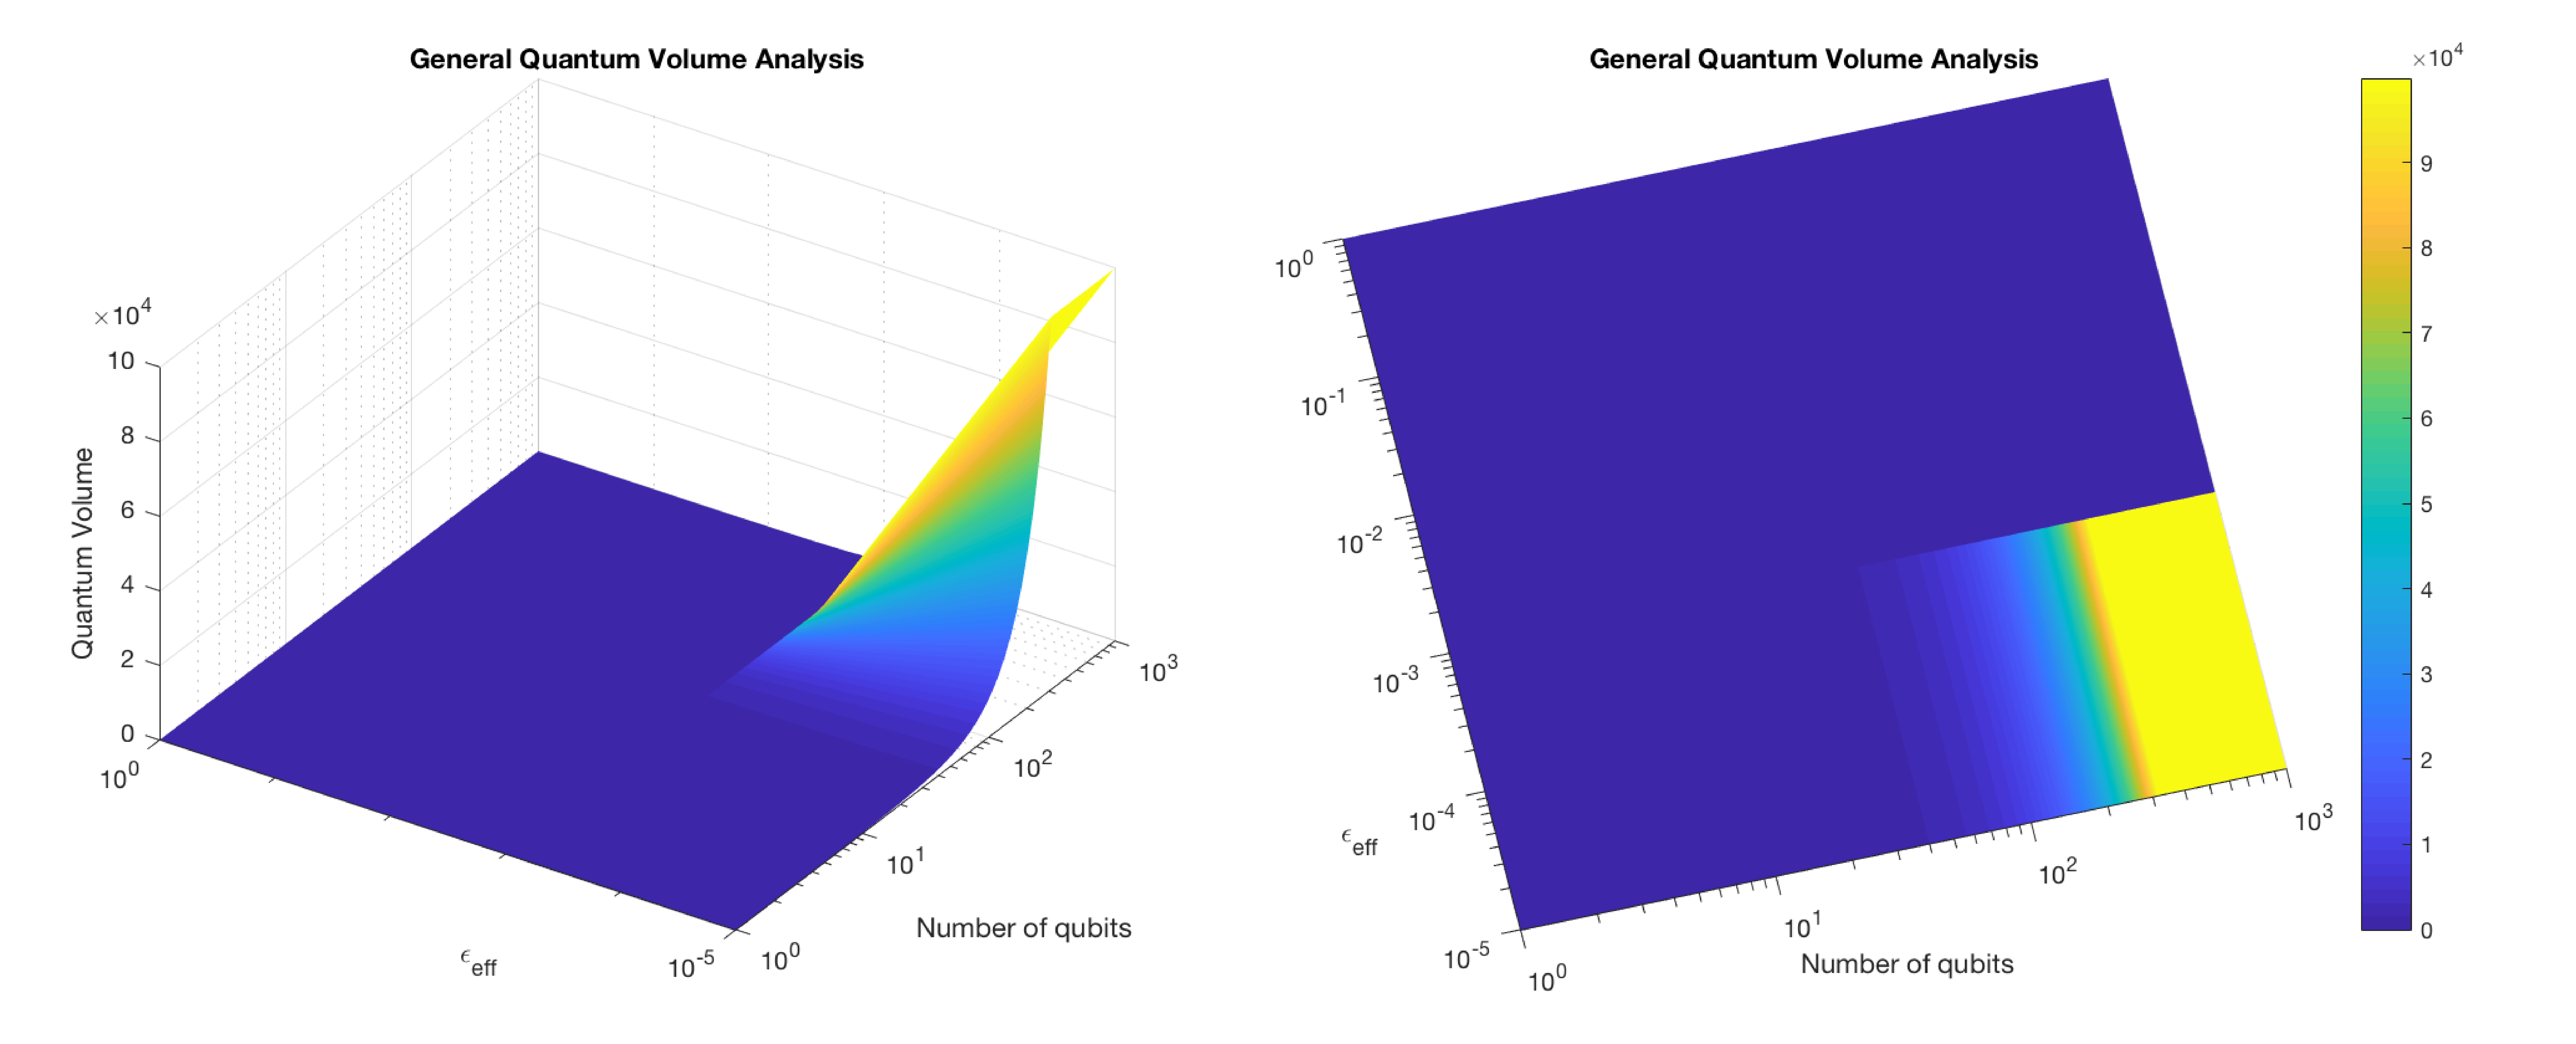
\includegraphics[width=\textwidth]{figures/general_QV.png}
\caption{\label{fig:orge67672d}
Device Quantum Volume behaviour for values less than 1000 qubits and a \(\epsilon_eff < 10^{-5}\)}
\end{figure}

\item Quantum Volume of an algorithm
\label{sec:org9fa755a}

As with \(V_Q\), we initially defined the algorithm's Quantum Volume from the general equation \(\tilde{V}_Q\), although we will adapt it later.

\begin{equation}
\label{eq:orgc799c10}
V_Q^a = \min \left[ n,d \right]^2
\end{equation}

Note that \(d\) is not \(d(N)\) but the real depth of the given algorithm.
At the same time, \(n\) is the number of qubits required by the algorithm itself.
One can see how \(d\) and \(n\) are equally important in Fig. \ref{fig:algorithmQVsym}.
The growth of both variables causes an equally exponential growth of \(V^a_Q\).

\begin{figure}[htbp]
\centering
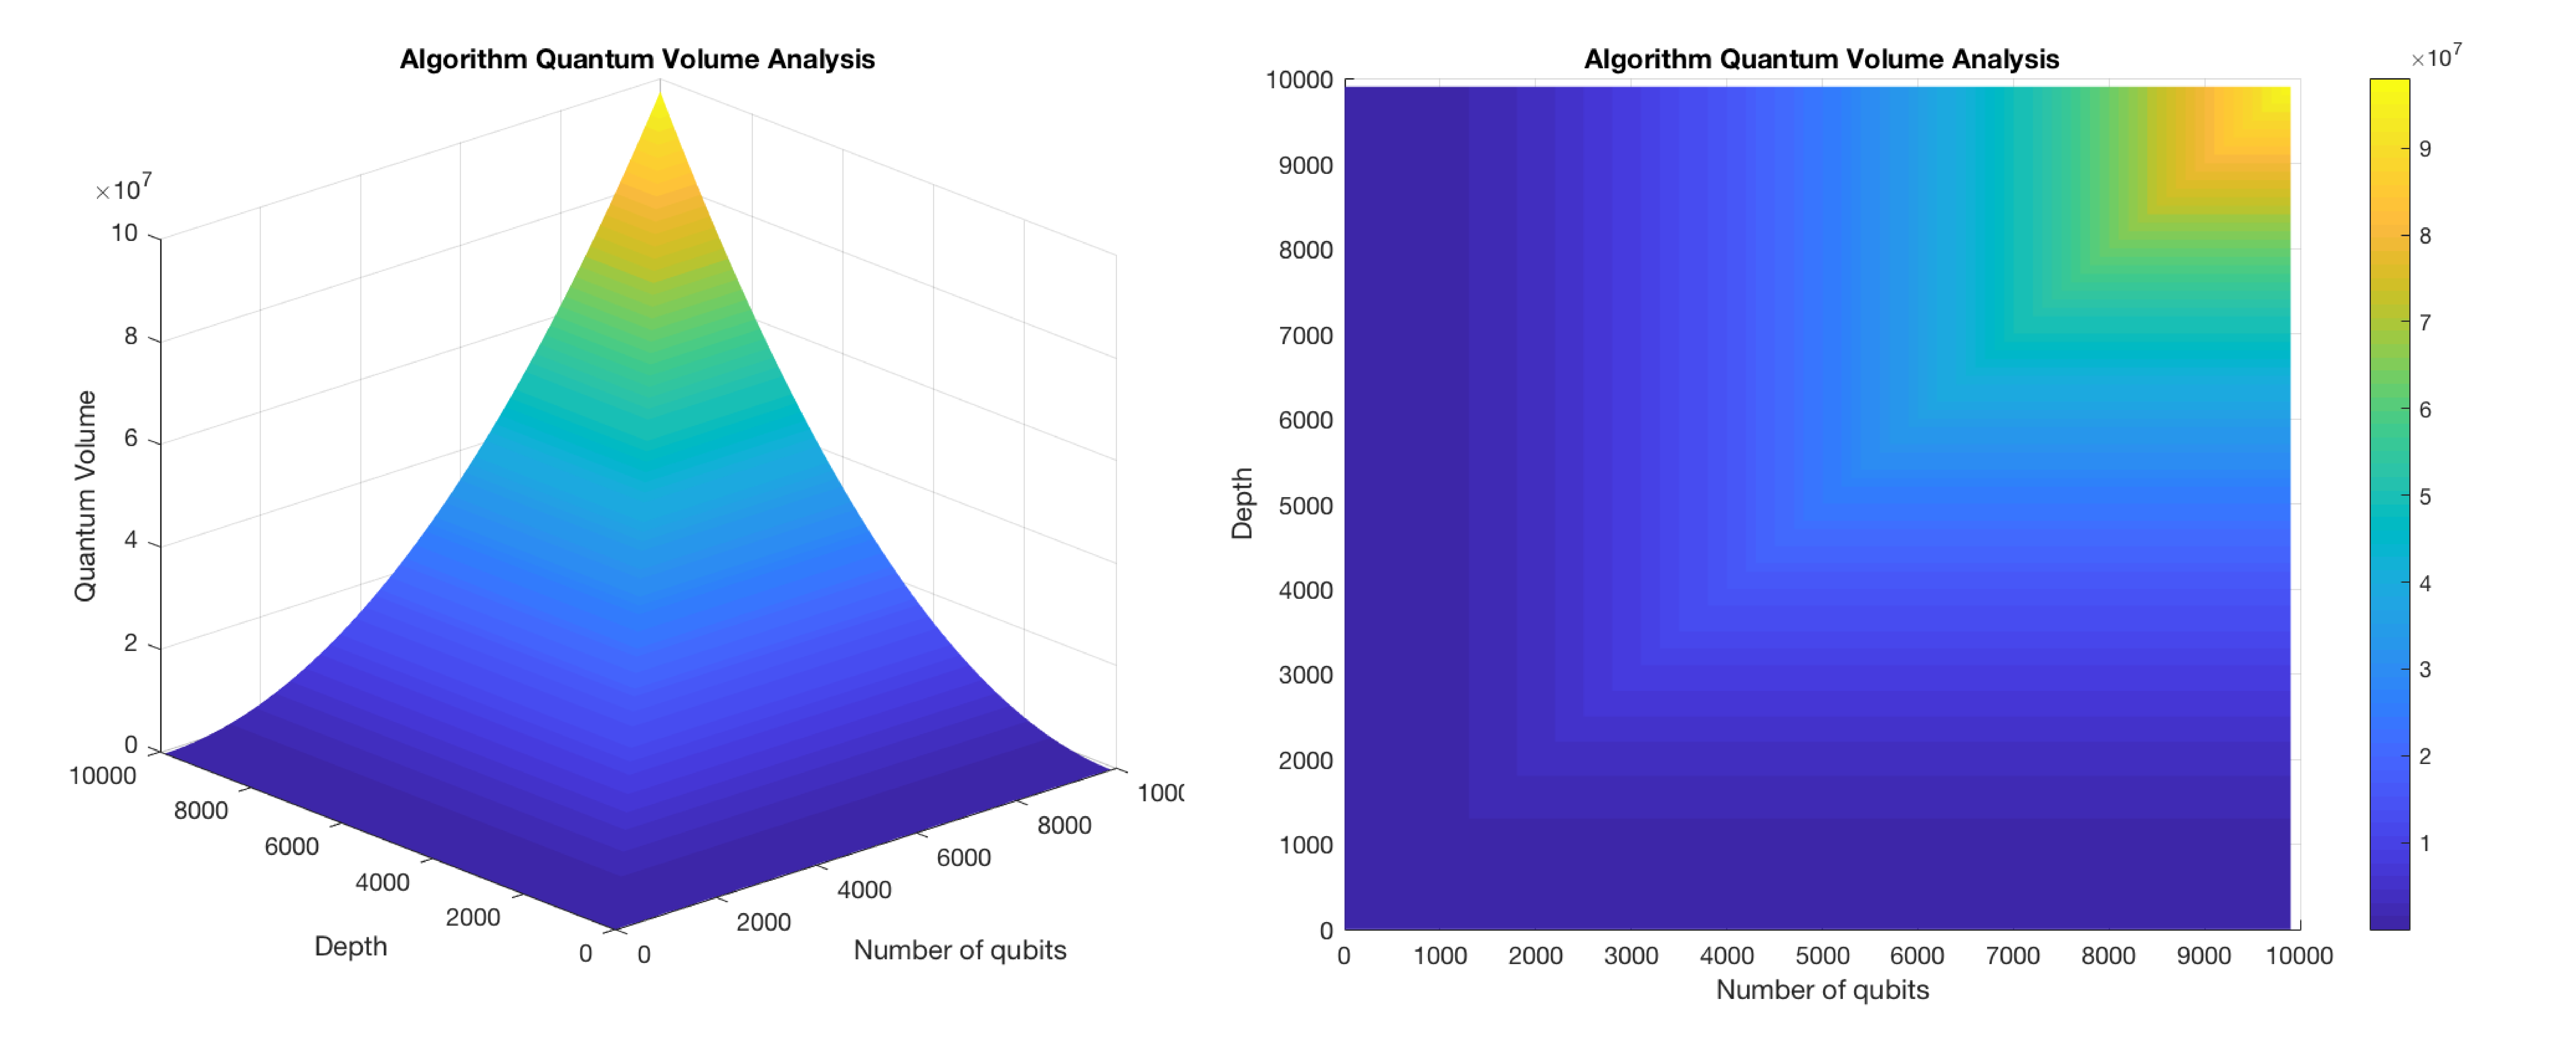
\includegraphics[width=\textwidth]{figures/V_q_analysis_sym.png}
\caption{\label{fig:org82080b1}
Algorithm Quantum Volume as in eq. \ref{eq:orgc799c10} behaviour for values less than \(10^{4}\) qubits and depth less than \(10^{4}\)}
\end{figure}

Fig. \ref{fig:algorithmQVasym} present the behaviour of \(V_Q^a\)
focusing in the current most common values for \(n\) and \(d\).
The function shows an asymteric beheviour due to \(d\) is much bigger than \(n\) most of the times.


\begin{figure}[htbp]
\centering
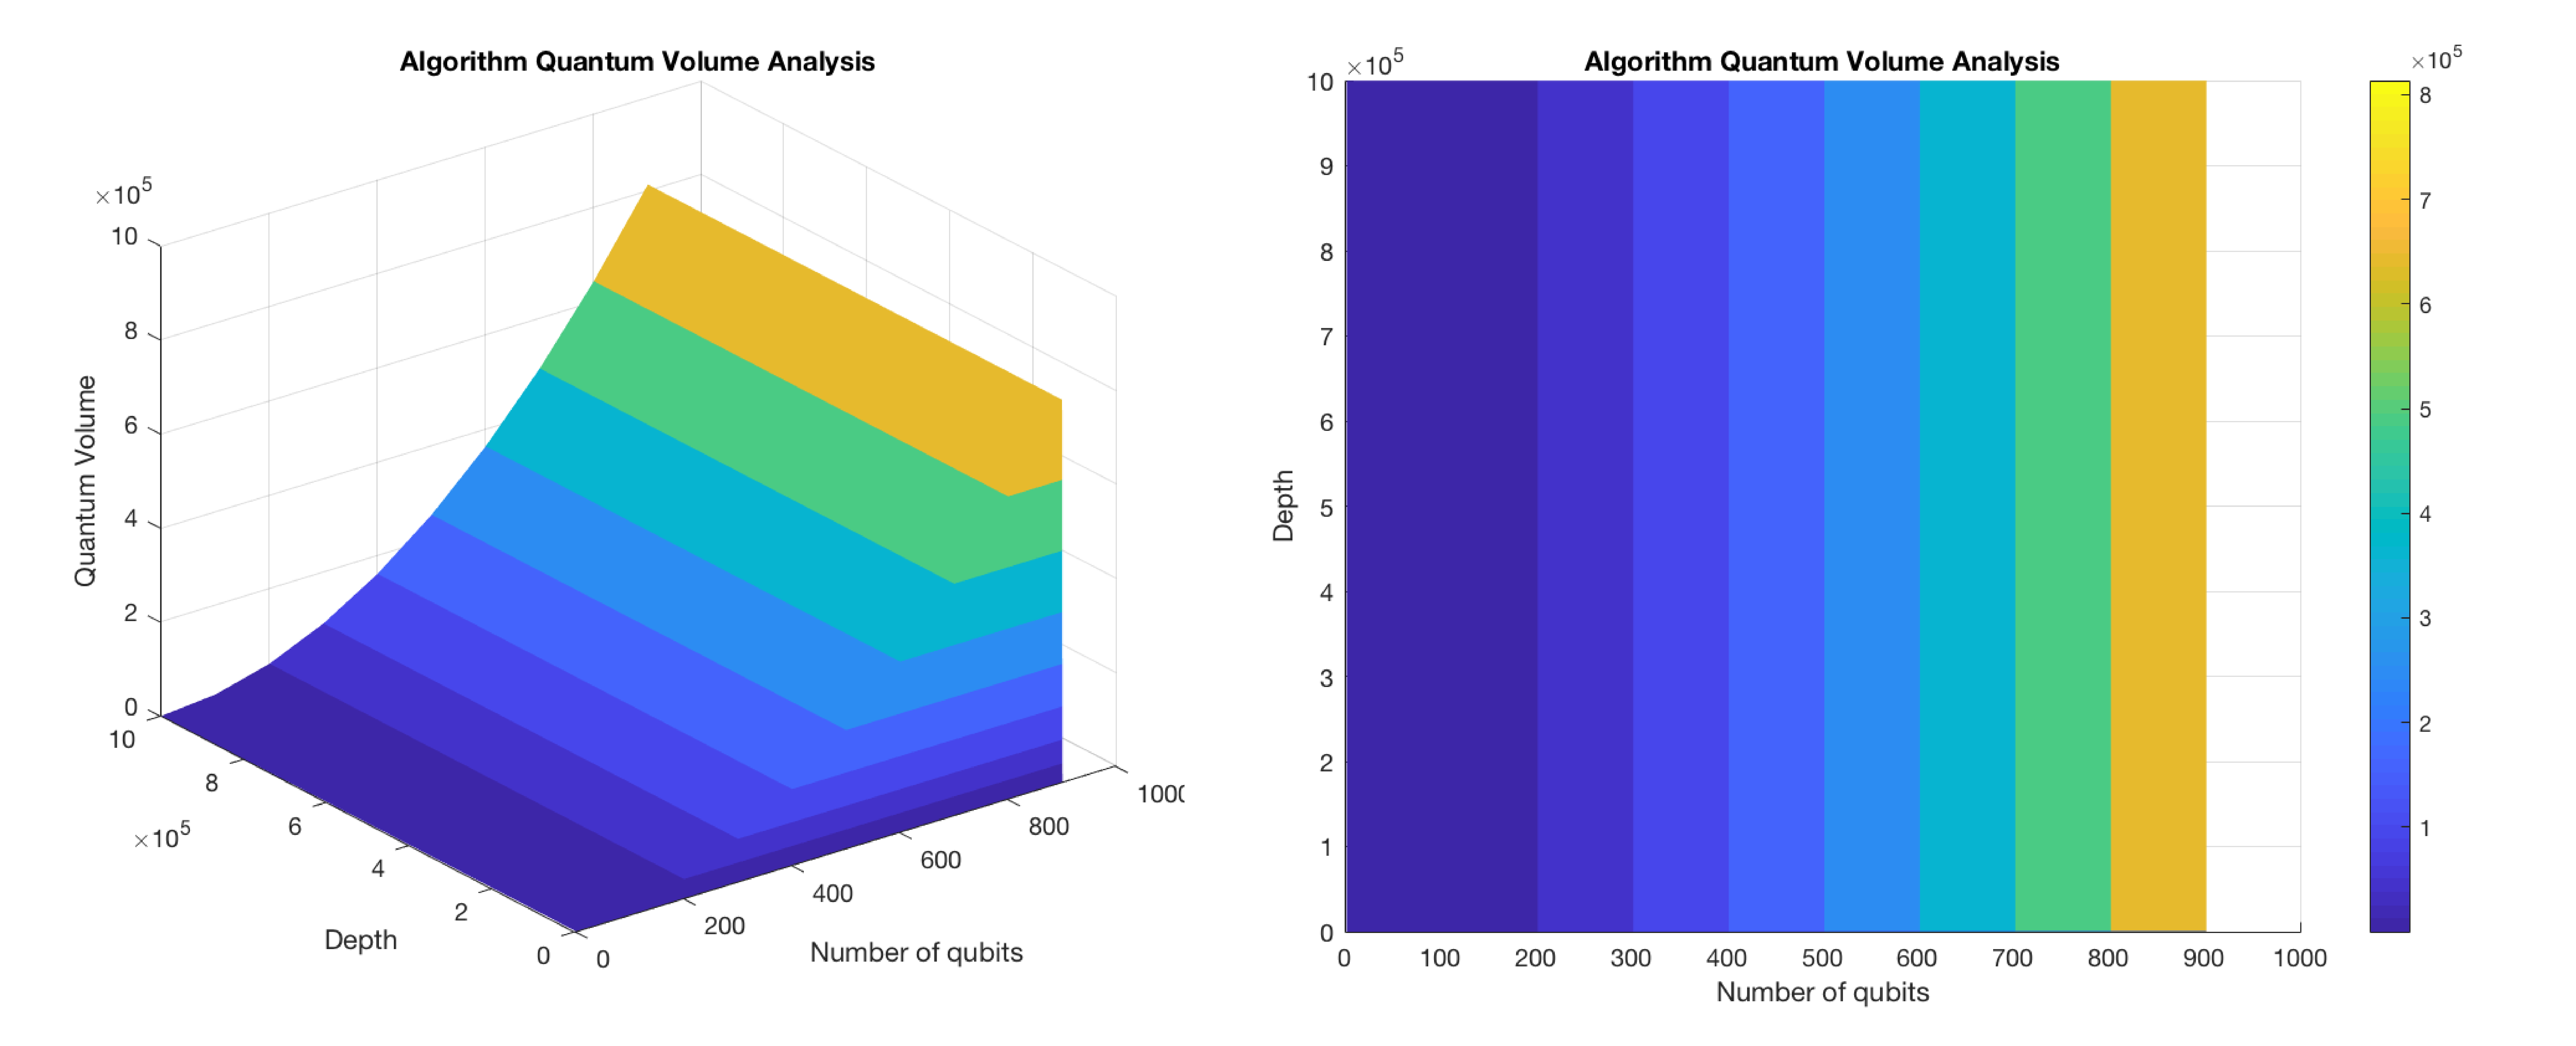
\includegraphics[width=\textwidth]{figures/V_q_analysis_asym.png}
\caption{\label{fig:orgf2ba1b3}
Algorithm Quantum Volume as in eq. \ref{eq:orgc799c10} behaviour for values less than 1000 qubits and a depth less than \(10^{5}\)}
\end{figure}

We aware that this approach has a limitation regarding the mapping of the quantum circuit.
As explained before, \(V_Q\) is able to take into account the sophistication of the mapping procedure.
It is inherited in the \emph{model algorithm}.
But, in this case, the \(V^a_Q\) of an algorithm before and after mapping will remain the same.
After mapping an algorithm, the usual effect is an increase in the depth or the number of operations.
Rare mapping methods consider the qubit addition in the technique.
And, even considering it, \(n\) is not often growing too much in comparison with \(d\).
In the current NISQ era, the quantum circuits need much less qubits than depth.
Therefore, most of the times, the minimum value between \(n\) and \(d\) will be \(n\).
As soon as \(V^a_Q\) is taking into account the minimum of them and the mapping procedure affects mostly to \(d\) we can conclude that this definition of \(V^a_Q\) is not considering the mapping in its results.

A simplified solution for this problem would be the \(V^a_Q\) definition as the multiplication between \(n\) and \(d\).
Unfortunately, this approach has several drawbacks as well.
As Moll et al. point out \cite{Moll_2018}, extreme cases of high \(n\) and low \(d\) -- or the other way around -- lead to inconsistencies of the multiplication metric.
But, considering that most of our work is not going to be in any of these extreme cases and that we can avoid those outliers, we define the algorithm's Quantum Volume as:

\begin{equation}
\label{eq:org6aba4aa}
V_Q^a =  n \times d
\end{equation}

Fig. \ref{fig:algorithmmultQV} report the behaviour of the \(V_Q^a\) as
the multiplication of \(n\) and \(d\).
As illutrated in Fig. \ref{fig:algorithmQVsym}, the values of \(n\) and \(d\) are
affecting equally and exponentially to the metric.

\begin{figure}[htbp]
\centering
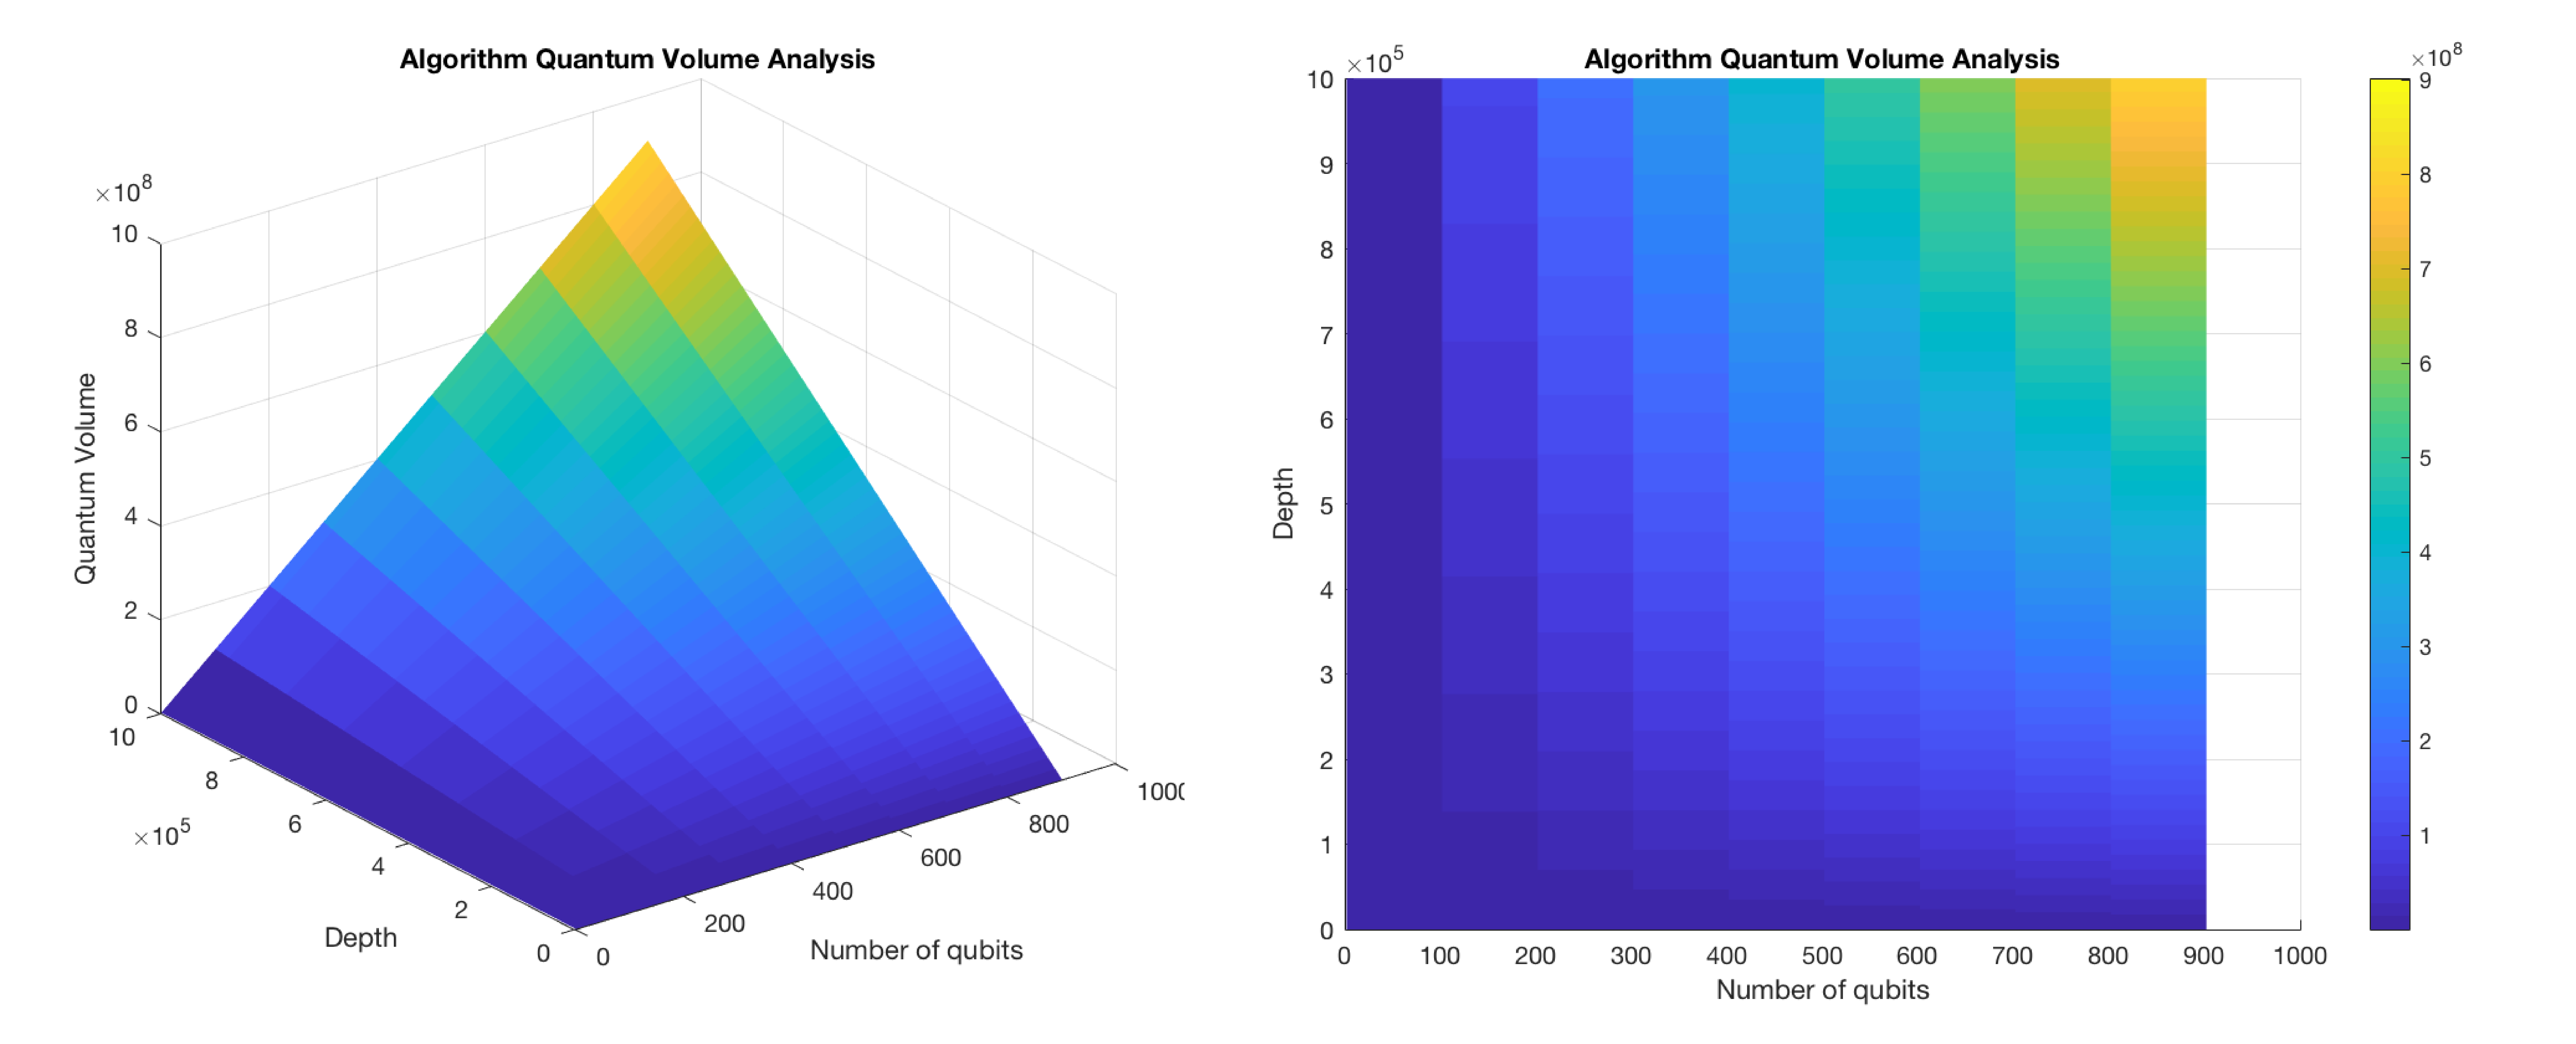
\includegraphics[width=\textwidth]{figures/V_q_analysis_mult.png}
\caption{\label{fig:org414674c}
Algorithm Quantum Volume as in eq. \ref{eq:org6aba4aa} behaviour for values less than 1000 qubits and a depth less than \(10^{5}\)}
\end{figure}

\item Runnability
\label{sec:org3254303}

Finally, once the Quantum Volume of device and algorithm are stated, we define runnability as the condition for which the \(V_Q\) should be bigger than \(V^a_Q\).
That is the condition that the computational power of the device should be bigger than the computational power required by the algorithm.

$$\text{Runnable if: } V_Q > V^a_Q \quad \quad \text{ when } N \ge n$$

For instance, in order to understand this concept, one may imagine the process of checking, whether or not, some cube with a given volume -- representing the algorithm -- would fit in a box -- the device --.
If the algorithm's box volume is smaller than the volume of the device's box, the algorithm's box will fit inside.

Indeed, one acceptable criticism of this definition is that, as \(V_Q\) and \(V^a_Q\) are finally defined in the previous sections, it seems that it is not really fair to compare them.
But, as soon as the general behaviour of the final and the initial \(V^a_Q\) is the same -- one can see in the Fig. \ref{fig:algorithmQVsym} and Fig. \ref{fig:algorithmmultQV} -- and as the final definition tends to have bigger values than the initial one -- so it is defining a more restrictive and exigent scenario -- we believe that this definition of runnability is mathematically correct and useful.

Therefore, we define runnability as the condition of:

\begin{equation}
\label{eq:orge149198}
\max_{n \le N} \min \left[ n,\frac{1}{n \epsilon_{eff} (n)}\right]^2 > n \times d \quad \quad \text{ when } N \ge n
\end{equation}
\end{enumerate}
\end{enumerate}

\item Methodology
\label{sec:org2d3f496}

After explaining the insights and our new concepts around the metric of Quantum Volume, let us now
look at our methodology.
One issue that needs to be raised is the difficulty of the \(\epsilon_{eff}\) calculation for a device.
In our work, we will try to avoid this exhausting process outlining how much computational power
is required by a given algorithm.
Or, in other words, we will calculate the \(V^a_Q\) and assert that it would be able to run in devices
with \(V_Q > V^a_Q\).
\(V^a_Q\) will be a threshold to define the runnability of a given algorithm.

As mentioned at the beginning, we are also interested on the impact of the mapping step in the
Quantum Volume.
Because of that, we will check the differences of \(V^a_Q\) in the same circuit, before and after
mapping it.
We are concerned about the relation between Quantum Volume and the probability of success, as
well.
We will analyze the results of both metrics, thus.

Subsequently, the design of our Quantum Volume method will follow the next stages.
First, given a quantum algorithm, we will calculate the Quantum Volume of a circuit, before and after mapping.
Then, we will compare both results and we will investigate their relationship with the probability
of success, if any.
Finally, we will outline the runnability threshold of the algorithm.

\begin{table}[htbp]
\caption{\label{tab:orga611381}
Summary of the steps to outline the range of possible values for running a given algorithm}
\centering
\small
\begin{tabular}{|l|}
\hline
\\
Steps:\\
\\
1. Calculation of \(V^a_Q \prime\) for a given algorithm without mapping\\
2. Calculation of \(V^a_Q\) for a given algorithm after being mapped with the constraints of some device\\
3. Compare \(V^a_Q \prime\) and \(V^a_Q\)\\
4. Look for relation with probability of success\\
5. Threshold \(V_Q\) with \(V^a_Q\) (\(V_Q > V^a_Q\) and \(N \ge n\))\\
\\
\hline
\end{tabular}
\end{table}
\end{enumerate}
